\documentclass[11pt,a4paper]{article}

% Packages
\usepackage[margin=2.5cm]{geometry}
\usepackage{microtype}
\usepackage{graphicx}
\usepackage{tikz}
\usetikzlibrary{shapes,arrows.meta,positioning,calc,fit,backgrounds,shadows.blur,decorations.pathmorphing,decorations.pathreplacing}
\usepackage{colortbl}
\usepackage{enumitem}
\usepackage{booktabs}
\usepackage{longtable}
\usepackage{hyperref}
\usepackage{xcolor}
\usepackage{fancyhdr}
\usepackage{titlesec}
\usepackage[most]{tcolorbox}
\usepackage{multicol}
\usepackage{amsmath,amssymb}
\usepackage{multirow}
\usepackage{setspace}
\usepackage{fontawesome5}
\usepackage{listings}

% Spacing
\setlength{\parskip}{3pt plus 1pt minus 1pt}
\setlength{\parindent}{0pt}

% Colors
\definecolor{primary}{HTML}{1A5276}
\definecolor{secondary}{HTML}{2E86C1}
\definecolor{accent}{HTML}{E74C3C}
\definecolor{lightbg}{HTML}{EBF5FB}
\definecolor{defbg}{HTML}{FDF2E9}
\definecolor{greenhl}{HTML}{27AE60}
\definecolor{purplehl}{HTML}{8E44AD}
\definecolor{codebg}{HTML}{F4F6F7}

% Hyperref
\hypersetup{colorlinks=true, linkcolor=primary, urlcolor=secondary, citecolor=primary}

% Code listings style
\lstset{
  backgroundcolor=\color{codebg},
  basicstyle=\ttfamily\small,
  keywordstyle=\color{primary}\bfseries,
  stringstyle=\color{greenhl},
  commentstyle=\color{gray},
  breaklines=true,
  frame=l,
  framerule=2pt,
  rulecolor=\color{secondary!40},
  xleftmargin=8pt,
  framexleftmargin=6pt,
  aboveskip=6pt,
  belowskip=6pt,
  showstringspaces=false,
  language=Python
}

% Header/Footer
\pagestyle{fancy}
\fancyhf{}
\fancyhead[L]{\small\textcolor{primary}{\textbf{Generative AI --- Core Concepts}}}
\fancyhead[R]{\small\textcolor{primary}{Lecture Handout}}
\fancyfoot[C]{\small\thepage}
\renewcommand{\headrulewidth}{0.5pt}
\renewcommand{\footrulewidth}{0.3pt}

% Section formatting
\titleformat{\section}{\Large\bfseries\color{primary}}{\thesection}{0.6em}{}[\vspace{2pt}\titlerule]
\titleformat{\subsection}{\large\bfseries\color{secondary}}{\thesubsection}{0.5em}{}
\titleformat{\subsubsection}{\normalsize\bfseries\color{primary}}{\thesubsubsection}{0.5em}{}
\titlespacing*{\section}{0pt}{14pt}{8pt}
\titlespacing*{\subsection}{0pt}{10pt}{5pt}

% Custom boxes
\newtcolorbox{definitionbox}[1][]{
  enhanced, breakable,
  colback=defbg, colframe=orange!60!black,
  colbacktitle=orange!70!black, coltitle=white,
  title={\faIcon{book}~#1}, fonttitle=\bfseries,
  boxrule=0pt, leftrule=4pt, arc=2pt,
  shadow={1mm}{-1mm}{0mm}{black!15},
  top=4pt, bottom=4pt, left=8pt, right=8pt
}
\newtcolorbox{conceptbox}[1][]{
  enhanced, breakable,
  colback=lightbg, colframe=secondary,
  colbacktitle=secondary, coltitle=white,
  title={\faIcon{lightbulb}~#1}, fonttitle=\bfseries,
  boxrule=0pt, leftrule=4pt, arc=2pt,
  shadow={1mm}{-1mm}{0mm}{black!15},
  top=4pt, bottom=4pt, left=8pt, right=8pt
}
\newtcolorbox{alertbox}[1][]{
  enhanced, breakable,
  colback=red!4, colframe=accent,
  colbacktitle=accent, coltitle=white,
  title={\faIcon{exclamation-triangle}~#1}, fonttitle=\bfseries,
  boxrule=0pt, leftrule=4pt, arc=2pt,
  shadow={1mm}{-1mm}{0mm}{black!12},
  top=3pt, bottom=3pt, left=8pt, right=8pt
}
\newtcolorbox{examplebox}[1][]{
  enhanced, breakable,
  colback=green!4, colframe=greenhl,
  colbacktitle=greenhl, coltitle=white,
  title={\faIcon{code}~#1}, fonttitle=\bfseries,
  boxrule=0pt, leftrule=4pt, arc=2pt,
  shadow={1mm}{-1mm}{0mm}{black!12},
  top=3pt, bottom=3pt, left=8pt, right=8pt
}

\begin{document}

% Title
\begin{center}
\vspace*{0.5cm}
{\Huge\bfseries\textcolor{primary}{Generative AI}}\\[8pt]
{\Huge\bfseries\textcolor{primary}{Core Concepts and Basics}}\\[16pt]
{\color{secondary}\rule{0.6\textwidth}{1.5pt}}\\[14pt]
{\Large\textsc{BSIT Data Science Lecture Handout}}\\[8pt]
{\large\textcolor{gray!70!black}{Models $\bullet$ Prompts $\bullet$ LLMs $\bullet$ Diffusion $\bullet$ Responsible Use}}
\vspace{0.3cm}
\end{center}

\tableofcontents
\newpage

%=============================================================
\section{Introduction to Generative AI}
%=============================================================

\begin{definitionbox}[Generative AI]
Generative AI is a branch of artificial intelligence that can \textbf{create new content} such as text, images, audio, code, video, and synthetic data. Instead of only classifying or predicting labels, it learns patterns from existing data and produces new outputs that resemble that data.
\end{definitionbox}

\begin{conceptbox}[Simple Meaning]
If a model can write a paragraph, create an image from a prompt, complete computer code, summarize a document, or generate a voice clip, it is acting as a \textbf{generative} model.
\end{conceptbox}

\subsection{Where Generative AI Fits}

\begin{center}
\begin{tikzpicture}[scale=1]
  \fill[black!8] (0.08,-0.08) circle (4.7cm);
  \fill[blue!6] (0,0) circle (4.7cm);
  \draw[thick, primary, line width=1.5pt] (0,0) circle (4.7cm);
  \node[font=\bfseries\large, primary] at (0,4.0) {\faIcon{robot}~Artificial Intelligence};
  \node[font=\scriptsize, primary!70, align=center] at (3.4,-3.3) {Expert systems,\\search, planning,\\recommendation};

  \fill[orange!8] (0,-0.4) circle (3.0cm);
  \draw[thick, orange!70!black, line width=1.2pt] (0,-0.4) circle (3.0cm);
  \node[font=\bfseries, orange!70!black] at (0,2.1) {\faIcon{brain}~Machine Learning};
  \node[font=\scriptsize, orange!50!black, align=center] at (-2.2,0.25) {Classification,\\regression,\\clustering};

  \fill[green!8] (0,-0.7) circle (1.65cm);
  \draw[thick, greenhl!70!black, line width=1.2pt] (0,-0.7) circle (1.65cm);
  \node[font=\bfseries\small, greenhl!70!black, align=center] at (0,-0.7) {\faIcon{magic}\\Generative\\AI};
\end{tikzpicture}
\end{center}

\begin{itemize}[leftmargin=*]
  \item \textbf{AI} is the broad field of making machines behave intelligently.
  \item \textbf{Machine Learning} learns patterns from data.
  \item \textbf{Generative AI} focuses on creating new outputs based on learned patterns.
\end{itemize}

\subsection{Why Generative AI Matters}

\begin{itemize}[leftmargin=*]
  \item It helps people create content faster.
  \item It supports chatbots, digital assistants, coding tools, design tools, and educational tools.
  \item It is widely used in text generation, image generation, translation, summarization, and content personalization.
  \item It is transforming how humans interact with software.
\end{itemize}

%=============================================================
\section{Generative AI vs. Traditional Predictive AI}
%=============================================================

\begin{center}
\begin{tabular}{@{}p{4.1cm}p{4.1cm}p{4.4cm}@{}}
\toprule
\textbf{Aspect} & \textbf{Predictive / Discriminative AI} & \textbf{Generative AI} \\
\midrule
Main goal & Predict labels or values & Create new content \\
Typical output & Class, score, forecast & Text, image, code, audio, video \\
Common question & ``What is this?'' & ``Create something like this'' \\
Examples & Spam detection, house price prediction & ChatGPT, image generators, code assistants \\
\bottomrule
\end{tabular}
\end{center}

\begin{conceptbox}[Easy Distinction]
If a model tells you whether an email is spam, that is predictive AI. If a model writes a new email for you, that is generative AI.
\end{conceptbox}

%=============================================================
\section{Core Building Blocks}
%=============================================================

\rowcolors{2}{white}{defbg}
\begin{longtable}{@{}p{3.6cm}p{9.9cm}@{}}
\toprule
\rowcolor{primary!15}
\textbf{Concept} & \textbf{Meaning} \\
\midrule
\endhead
Prompt & The instruction or input given to the model \\
\addlinespace
Token & A small unit of text such as a word, part of a word, or symbol \\
\addlinespace
Embedding & A numeric representation that captures meaning or similarity \\
\addlinespace
Model & The trained system that generates outputs \\
\addlinespace
Parameter & A learned internal value of the model \\
\addlinespace
Inference & The stage where the model produces output for a new input \\
\addlinespace
Context window & The amount of input the model can consider at one time \\
\addlinespace
Temperature & A setting that affects randomness and creativity of the output \\
\addlinespace
Fine-tuning & Additional training to specialize a general model for a task or domain \\
\addlinespace
Multimodal model & A model that can work with more than one data type such as text and images \\
\bottomrule
\end{longtable}

\subsection{Tokens and Context}

\begin{definitionbox}[Token]
A token is a small piece of text processed by the model. A sentence is not read as one whole unit. It is split into smaller parts, and the model works through them step by step.
\end{definitionbox}

\begin{conceptbox}[Context Window]
The context window is like the model's working memory for the current interaction. If important information is outside that window, the model may ignore it or forget it.
\end{conceptbox}

\subsection{Embeddings}

\begin{definitionbox}[Embedding]
An embedding is a vector representation of data that places similar items close together in a mathematical space. In practice, this helps models compare meaning, search documents, recommend related items, and support retrieval systems.
\end{definitionbox}

%=============================================================
\section{How Generative AI Works}
%=============================================================

\subsection{Learning from Data}

\begin{conceptbox}[General Idea]
Generative models are trained on large collections of examples. During training, the model learns patterns such as grammar, style, structure, color relationships, sound patterns, or coding syntax. During use, it generates an output based on those learned patterns and the prompt it receives.
\end{conceptbox}

\subsection{Training, Fine-Tuning, and Inference}

\begin{center}
\begin{tikzpicture}[
  step/.style={rectangle, draw, thick, fill=#1, minimum width=2.5cm, minimum height=1.1cm, align=center, font=\footnotesize\bfseries, rounded corners=4pt,
    blur shadow={shadow blur steps=5, shadow xshift=0.5mm, shadow yshift=-0.5mm}},
  arr/.style={-{Stealth[length=2.5mm]}, very thick, primary!60, line width=1.15pt}
]
  \node[step=blue!12] (s1) at (0,0) {\faIcon{database}\\Training Data};
  \node[step=orange!12] (s2) at (3.3,0) {\faIcon{brain}\\Pretraining};
  \node[step=green!12] (s3) at (6.6,0) {\faIcon{sliders-h}\\Fine-Tuning};
  \node[step=red!10] (s4) at (9.9,0) {\faIcon{comment-dots}\\Inference};

  \draw[arr] (s1) -- (s2);
  \draw[arr] (s2) -- (s3);
  \draw[arr] (s3) -- (s4);
\end{tikzpicture}
\end{center}

\begin{itemize}[leftmargin=*]
  \item \textbf{Pretraining:} The model learns broad patterns from a very large dataset.
  \item \textbf{Fine-tuning:} The model is adapted to a specific domain, task, or style.
  \item \textbf{Inference:} The trained model is used to generate a response for a real user prompt.
\end{itemize}

\subsection{Text Generation Intuition}

\begin{definitionbox}[Next-Token Prediction]
Large language models often generate text by predicting the most suitable next token repeatedly. Over many steps, this creates a sentence, then a paragraph, then a complete answer.
\end{definitionbox}

\begin{examplebox}[Mini Example]
Prompt: \textit{``Write one sentence about data science.''}

The model does not retrieve one fixed sentence from memory. Instead, it generates the response token by token based on probabilities learned from training data and the current prompt.
\end{examplebox}

%=============================================================
\section{Main Families of Generative Models}
%=============================================================

\rowcolors{2}{white}{defbg}
\begin{longtable}{@{}p{3.2cm}p{3.2cm}p{6.3cm}@{}}
\toprule
\rowcolor{primary!15}
\textbf{Model Family} & \textbf{Common Output} & \textbf{Key Idea} \\
\midrule
\endhead
Large Language Models (LLMs) & Text, summaries, code, chat responses & Generate text token by token using transformer-based architectures \\
\addlinespace
Diffusion Models & Images, audio, video & Start from noise and gradually refine it into meaningful content \\
\addlinespace
GANs & Images, synthetic samples & A generator competes with a discriminator to create realistic outputs \\
\addlinespace
VAEs & Compressed or synthetic data & Learn a compact latent representation and generate samples from it \\
\bottomrule
\end{longtable}

\subsection{Large Language Models}

\begin{definitionbox}[LLM]
A Large Language Model is a generative model trained on large amounts of text. It can answer questions, summarize content, translate language, generate code, and hold conversations.
\end{definitionbox}

\subsection{Diffusion Models}

\begin{definitionbox}[Diffusion Model]
Diffusion models are widely used for image generation. They learn how to reverse noise. During generation, they begin with random noise and gradually transform it into a meaningful image that matches the prompt.
\end{definitionbox}

\subsection{GANs and VAEs}

\begin{itemize}[leftmargin=*]
  \item \textbf{GANs} use two networks: one generates content and the other judges whether it looks real.
  \item \textbf{VAEs} learn a compressed latent space and then generate samples from it.
  \item Both are important historically, even though modern text generation is dominated by transformer-based models.
\end{itemize}

%=============================================================
\section{Transformers and Attention}
%=============================================================

\begin{definitionbox}[Transformer]
The transformer is a neural network architecture that became the foundation of modern large language models. It is powerful because it can analyze relationships between different parts of the input efficiently.
\end{definitionbox}

\begin{conceptbox}[Attention]
Attention allows the model to focus on the most relevant words, symbols, or regions of the input when generating the next part of the output. This is why transformers are effective for long and complex sequences.
\end{conceptbox}

\begin{center}
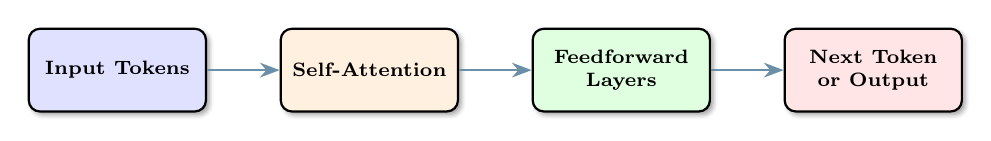
\begin{tikzpicture}[
  box/.style={rectangle, draw, thick, fill=#1, minimum width=2.25cm, minimum height=1.05cm, align=center, font=\scriptsize\bfseries, rounded corners=4pt,
    blur shadow={shadow blur steps=4, shadow xshift=0.4mm, shadow yshift=-0.4mm}},
  arr/.style={-{Stealth[length=2.5mm]}, thick, primary!65}
]
  \node[box=blue!12] (in) at (0,0) {Input Tokens};
  \node[box=orange!12] (attn) at (3.2,0) {Self-Attention};
  \node[box=green!12] (ffn) at (6.4,0) {Feedforward\\Layers};
  \node[box=red!10] (out) at (9.6,0) {Next Token\\or Output};

  \draw[arr] (in) -- (attn);
  \draw[arr] (attn) -- (ffn);
  \draw[arr] (ffn) -- (out);
\end{tikzpicture}
\end{center}

%=============================================================
\section{Prompting Basics}
%=============================================================

\begin{definitionbox}[Prompt]
A prompt is the instruction, question, context, or example given to a generative model in order to guide its output.
\end{definitionbox}

\subsection{What Makes a Good Prompt?}

\begin{itemize}[leftmargin=*]
  \item Be clear about the task.
  \item Provide enough context.
  \item State the desired format of the answer.
  \item Add constraints such as length, tone, or audience.
  \item Include an example when needed.
\end{itemize}

\begin{examplebox}[Prompt Engineering Example]
Weak prompt: \textit{``Explain AI.''}

Better prompt: \textit{``Explain generative AI to first-year BSIT students in five simple bullet points and include one real-life example.''}
\end{examplebox}

\subsection{Common Prompting Styles}

\rowcolors{2}{white}{defbg}
\begin{longtable}{@{}p{3.2cm}p{10.3cm}@{}}
\toprule
\rowcolor{primary!15}
\textbf{Prompting Style} & \textbf{Meaning} \\
\midrule
\endhead
Zero-shot & Ask the task directly without examples \\
\addlinespace
One-shot & Provide one example before asking for output \\
\addlinespace
Few-shot & Provide a few examples to guide the format or style \\
\addlinespace
Instruction prompting & Tell the model exactly what to do \\
\addlinespace
Role prompting & Ask the model to respond as a tutor, analyst, or assistant \\
\bottomrule
\end{longtable}

%=============================================================
\section{Retrieval, Grounding, and RAG}
%=============================================================

\begin{definitionbox}[Grounding]
Grounding means connecting the model to trusted information sources so its answers are based on real documents, databases, or knowledge rather than only what it learned during training.
\end{definitionbox}

\begin{definitionbox}[RAG --- Retrieval-Augmented Generation]
RAG combines information retrieval with generation. First, the system retrieves relevant content from a trusted source. Then, the model uses that retrieved content to generate a more accurate answer.
\end{definitionbox}

\begin{conceptbox}[Why RAG Is Useful]
RAG is helpful when we need more up-to-date or domain-specific answers, such as university policies, company documents, manuals, or course notes.
\end{conceptbox}

%=============================================================
\section{Applications of Generative AI}
%=============================================================

\begin{itemize}[leftmargin=*]
  \item \textbf{Text generation:} drafting reports, summaries, emails, and study notes.
  \item \textbf{Conversational systems:} virtual assistants, tutoring systems, and help desks.
  \item \textbf{Code generation:} suggesting functions, debugging help, and documentation.
  \item \textbf{Image generation:} marketing graphics, concept art, and design prototypes.
  \item \textbf{Audio generation:} speech synthesis, dubbing, and voice assistants.
  \item \textbf{Video generation:} short clips, explainers, and animation support.
  \item \textbf{Synthetic data:} generating additional training data when real data is limited or sensitive.
\end{itemize}

\subsection{Examples Relevant to BSIT Data Science}

\begin{examplebox}[Classroom-Relevant Use Cases]
\begin{itemize}[leftmargin=*]
  \item Generate study summaries from lecture notes.
  \item Create chatbot support for campus information.
  \item Assist with code explanation and documentation.
  \item Produce draft data reports from structured results.
  \item Generate synthetic examples for model testing and practice.
\end{itemize}
\end{examplebox}

%=============================================================
\section{Limitations and Risks}
%=============================================================

\begin{alertbox}[Generative AI Is Powerful but Not Perfect]
Generative models can sound confident even when they are wrong. They are useful assistants, but they are not guaranteed truth machines.
\end{alertbox}

\rowcolors{2}{white}{defbg}
\begin{longtable}{@{}p{3.2cm}p{4.0cm}p{6.1cm}@{}}
\toprule
\rowcolor{primary!15}
\textbf{Risk} & \textbf{What It Means} & \textbf{Possible Response} \\
\midrule
\endhead
Hallucination & The model invents incorrect facts & Verify with trusted sources and grounding \\
\addlinespace
Bias & Outputs may reflect unfair patterns in training data & Review data and test outputs carefully \\
\addlinespace
Privacy issues & Sensitive data may be exposed or mishandled & Avoid sharing private information in prompts \\
\addlinespace
Misinformation & Generated content may spread false claims & Human review before publishing or acting on outputs \\
\addlinespace
Overreliance & Users may trust the tool too much & Keep human judgment in the loop \\
\bottomrule
\end{longtable}

\subsection{Hallucination}

\begin{definitionbox}[Hallucination]
In generative AI, hallucination means the model produces content that sounds believable but is false, unsupported, or made up.
\end{definitionbox}

\subsection{Prompt Injection and Safety}

\begin{conceptbox}[Prompt Injection]
Prompt injection happens when malicious or misleading instructions try to manipulate a model or override its intended behavior. This matters when generative AI systems are connected to tools, files, or external data sources.
\end{conceptbox}

%=============================================================
\section{Evaluating Generative AI Systems}
%=============================================================

\begin{itemize}[leftmargin=*]
  \item \textbf{Relevance:} Does the answer address the prompt?
  \item \textbf{Accuracy:} Is the content factually correct?
  \item \textbf{Clarity:} Is the response easy to understand?
  \item \textbf{Groundedness:} Is the answer supported by source material?
  \item \textbf{Safety:} Does the output avoid harmful, biased, or toxic content?
  \item \textbf{Latency:} How quickly does the system respond?
\end{itemize}

\begin{conceptbox}[Human Evaluation Still Matters]
Unlike simple classification tasks, generative AI often needs human judgment because quality depends on context, usefulness, tone, and correctness.
\end{conceptbox}

%=============================================================
\section{Best Practices for Students and Developers}
%=============================================================

\begin{itemize}[leftmargin=*]
  \item Start with a clear use case.
  \item Use trusted data sources when accuracy matters.
  \item Write specific prompts instead of vague prompts.
  \item Validate important outputs before using them.
  \item Protect personal, confidential, and copyrighted data.
  \item Keep a human reviewer in the workflow.
  \item Compare model outputs with baseline methods when possible.
  \item Document how the system is used and what its limits are.
\end{itemize}

%=============================================================
\section{Mini Case Study for BSIT}
%=============================================================

\begin{definitionbox}[Campus Helpdesk Assistant]
Suppose a BSIT department wants to build a chatbot that answers common student questions about schedules, enrollment steps, laboratory rules, and course requirements.
\end{definitionbox}

\textbf{Possible design:}
\begin{enumerate}[leftmargin=*]
  \item Collect official FAQ documents and campus announcements.
  \item Store them in a searchable knowledge base.
  \item Use a generative model with RAG so answers are based on official documents.
  \item Add safety rules so the system does not invent policies.
  \item Let staff review important updates and monitor failures.
\end{enumerate}

\begin{alertbox}[Responsible Use]
For academic or administrative systems, generated answers should support staff and students, not replace official human approval where accuracy is critical.
\end{alertbox}

%=============================================================
\section{A Small API-Style Example}
%=============================================================

\begin{lstlisting}
prompt = "Summarize the topic Generative AI for BSIT students in 5 bullet points."

response = model.generate(
    prompt=prompt,
    temperature=0.4,
    max_tokens=200
)

print(response)
\end{lstlisting}

\begin{conceptbox}[What This Example Shows]
The prompt gives the task, the model generates text, and settings such as temperature and maximum tokens influence the style and length of the response.
\end{conceptbox}

%=============================================================
\section{Summary}
%=============================================================

\begin{itemize}[leftmargin=*]
  \item Generative AI creates new content such as text, images, code, and audio.
  \item It differs from predictive AI because its main goal is content creation, not only classification or forecasting.
  \item Core concepts include prompts, tokens, embeddings, context windows, inference, and fine-tuning.
  \item Important model families include LLMs, diffusion models, GANs, and VAEs.
  \item Transformers and attention are central to modern text-based generative AI.
  \item RAG helps improve accuracy by connecting the model to trusted external information.
  \item Generative AI has major benefits, but it also has risks such as hallucination, bias, and privacy problems.
\end{itemize}

%=============================================================
\section{Review Questions}
%=============================================================

\begin{enumerate}[leftmargin=*]
  \item What is generative AI, and how is it different from predictive AI?
  \item What is a prompt?
  \item What is a token, and why is it important in large language models?
  \item What is meant by a context window?
  \item What is the difference between pretraining, fine-tuning, and inference?
  \item How do LLMs differ from diffusion models?
  \item What does attention do in a transformer?
  \item What is hallucination in generative AI?
  \item Why is RAG useful in real applications?
  \item What ethical and practical risks should users consider when using generative AI?
\end{enumerate}

\end{document}